% This section describes our SMT approach for the Sports Tournament Scheduling (STS) problem, modeled using the Quantifier-Free Linear Integer Arithmetic (QF\_LIA) theory and solved with Z3 and CVC5.
% The approach is divided into two phases.

% In \textbf{Phase~1}, we generate a feasible schedule by selecting a valid assignment of precomputed matches to each slot. Weekly matches are determined in advance using the standard round-robin method. The feasibility constraints ensure that each slot contains exactly one valid pair, each pair is used exactly once, and every team respects participation limits.

% In \textbf{Phase~2}, we optimize the feasible solution by balancing the number of home and away games for each team. This is done by introducing flip variables that can invert the home and away teams in each match to reduce imbalance. Each phase is encoded in a separate \texttt{.smt2} file: the first finds a valid solution, the second refines it by minimizing imbalance.

\subsection{Decision Variables}

\textbf{Phase~1:}
\begin{itemize}
    \item $\mathit{home}_{p,w} \in \{1,\dots,n\}$: team playing at home in period $p$, week $w$.
    \item $\mathit{away}_{p,w} \in \{1,\dots,n\}$: team playing away in period $p$, week $w$.
    \item $\mathit{index}_{p,w,t} \in \{ \text{true}, \text{false} \}$: true if pair $t$ is assigned to slot $(p,w)$.
\end{itemize}

\textbf{Phase~2:}
\begin{itemize}
    \item $\mathit{flip}_{p,w} \in \{ \text{true}, \text{false} \}$: true if the home and away teams in slot $(p,w)$ are swapped to improve balance.
    \item $\mathit{homeEff}_{p,w}$, $\mathit{awayEff}_{p,w}$: effective home and away teams after applying flips.
\end{itemize}

\subsection{Objective Function}

The objective function applies only to \textbf{Phase~2} and aims to minimize the maximum imbalance $k$ between home and away games for any team:
\[
k^* = \min \{ k : \forall t,\, |H_t - A_t| \leq k \},
\quad H_t = \sum_{p,w} [\mathit{homeEff}_{p,w} = t], \quad
A_t = \sum_{p,w} [\mathit{awayEff}_{p,w} = t].
\]

The effective assignments are the following.
\[
\mathit{homeEff}_{p,w} = \text{ite}(\mathit{flip}_{p,w},\, \mathit{away}_{p,w},\, \mathit{home}_{p,w}), \quad
\mathit{awayEff}_{p,w} = \text{ite}(\mathit{flip}_{p,w},\, \mathit{home}_{p,w},\, \mathit{away}_{p,w}).
\]

The optimal $k^*$ is found using a binary search over feasible imbalance bounds.

\subsection{Constraints}

\textbf{Phase~1:}
\begin{itemize}
    \item \textbf{Pair selection:} each slot $(p,w)$ selects exactly one valid pair:
    \[
    \bigvee_{t} \Big(
        \mathit{index}_{p,w,t} \wedge
        \mathit{home}_{p,w} = h_{t,w} \wedge
        \mathit{away}_{p,w} = a_{t,w}
    \Big).
    \]
    \item \textbf{Unique pair usage:} each pair appears exactly once:
    \[
    \sum_{p} \mathit{index}_{p,w,t} = 1, \quad \sum_{w} \mathit{index}_{p,w,t} = 1.
    \]
    \item \textbf{Period participation limit:} each team appears at most twice in the same period over the tournament.
    \item \textbf{Symmetry breaking:} the first pair is fixed: $\mathit{index}_{0,0,0} = \text{true}$.
\end{itemize}

\textbf{Phase~2:}
\begin{itemize}
    \item \textbf{Balance condition:}
    \[
    |H_t - A_t| \leq k, \quad \forall t.
    \]
\end{itemize}
\textit{Note:} all feasibility constraints from Phase~1 remain implicitly valid, since Phase~2 only modifies the home/away role through flips but does not change the original match assignments.


\subsection{Validation}
\begin{figure}[h!]
  \centering
  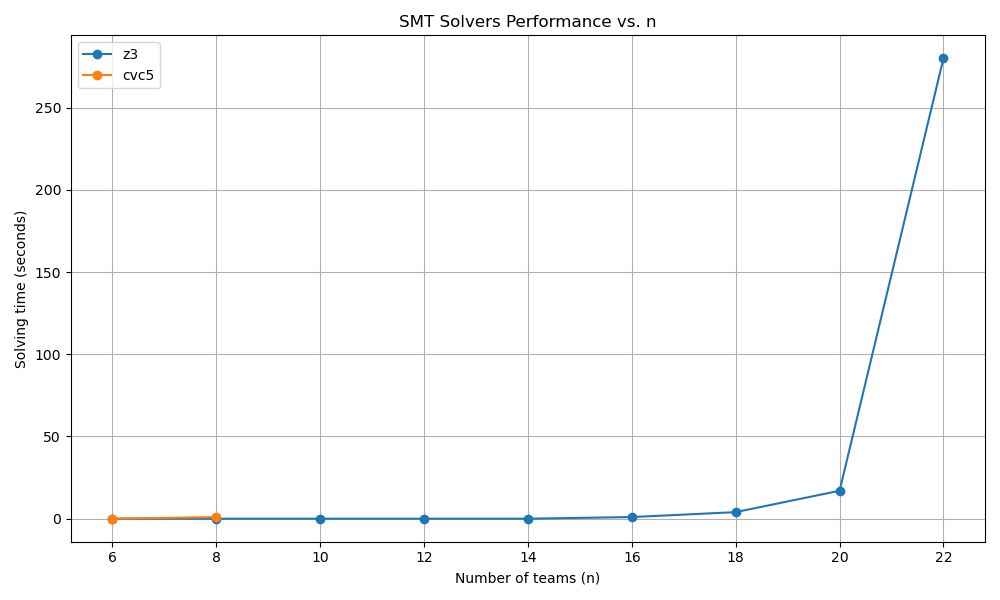
\includegraphics[width=0.8\textwidth]{img/SMT-result.png}
  \caption{}
  \label{fig:output}
\end{figure}